\chapter{Relevante Grundlagen und Überblick den alternativen Antrieben}
\label{ch:Relevante Grundlagen und Überblick den alternativen Antrieben}

\section{Bodenabfertigung eines Flugzeugs}
\label{s:Bodenabfertigung eines Flugzeugs}

\section{Stakeholder am Flughafen und deren Teil an der Abfertigung}


Referenz-Verlauf
Schmidt 2016 
According to requirements stated in EU-OPS 1.305 (FAR 121.570)
 (European Commission, 2008), the aircraft is refueled once the last
 passenger has left the aircraft.


Mensen definiert die Abfertigung, als Akteure am Flughafen, wie Flugplatzbetreieber, Fluggesselschaft und die Dritte mit einem Ziel ein 
Flugzeug zu nächstem Flug vorzubereiten. 

Kurz aus Mensen:
Der Ablauf eines Turn Around beginnt am Parkposition der Flughafen. Die Triebwerke werden ausgeschaltet 
und das Flugzeug an auxiliary power unit (APU) angeschlossen, APU liefert Strom, wenn die Haupttriebwerke nicht laufen. 
[Annex 14. Doc 9137 Part 8]  
Fracht (ULD) wird mit dem Hubwagen abgeladen und mit Dollies aus Transporthängern zur Sortieranlage im Terminal gebracht \cite{mensen2013handbuch}.
Parallel ist den Förderband für einzelne Gepäckstücke und Sperrgepäck benutzt, Passagiere über oder Treppe zum Bus aussteigen.
Nach dem Aussteigen aller Passagiere darf es mit der Betankung angefangen werden. 
Nach der Reinigung der Kabine (Boeing B747-400 im Transit bis zu 45 min), Toiletten und Frischwasser nachfüllen und Catering
Boarding ca. 15-20 min pro 100 PAX

Im Weiteren ist eine Abfertigung des Flugzeugs beschrieben, ohne Vorkommnisse und für ein gutes Wetter.
Wenn ein Flugzeug landet und auf seine Parkposition rollt und einen Block hingelegt wird beendet die Blockzeit eines Fluges, 

Das Flugzeug wird abgefertigt und wenn die Flüge zeitnan zusammen liegen beginnt ein Turn Around (TA) \cite{mensen2013handbuch}, 
d.h. das Flugzeug durch viele Akteure am Flughafen, wie Flugplatzbetreieber, Fluggesselschaft und die Dritte, für 
nächsten Flug vorbereitet wird \cite{mensen2013handbuch}.
Es muss ausgeladen, kontrolliert, gereinigt und dann versorgt und für den nächsten Flug beladen werden. 

\begin{figure}[h]
	\centering
	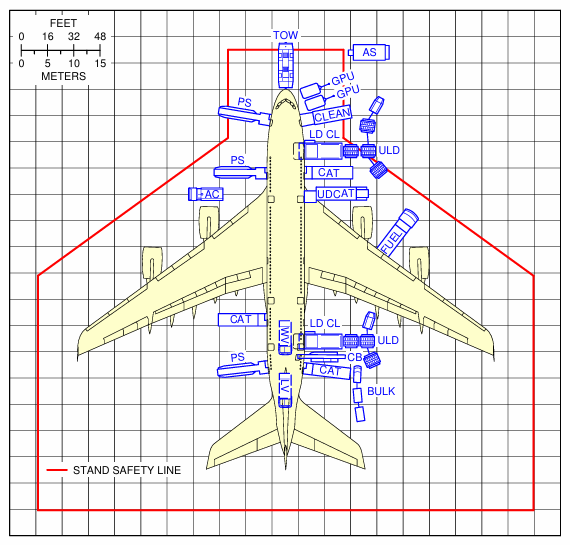
\includegraphics[width=0.8\linewidth]{Bilder/A380.png}
	\caption[Abfertigung A380]{Abfertigung eines A380 \cite{AirbusA380Characteristics}}
	\label{abfertigung}
\end{figure}


"Die
TurnaroundTime ist die Zeit vom Andocken des Flugzeugs amGate bis zumAbrollen
vomGate." \cite{conrady2019luftverkehr} S 368

Abfertigung Frachtflugzeug?
Nach Mensen werden folgend geteilt S. 1133:

Fluggast- Fracht-, und Postabfertigung 
Fluggastabfertigung beinhaltet alles um den Service für die Passagiere.

Vorfelddienste

Betankungsdienste führen nicht nur die Be- und Entladung und Lagerung durch, sondern auch für andere Flüssigkeiten (wie z.B. Öl) zuständig.
Wartungsdienste führen die routinemäßige Kontrolle den Flugzeugen vor den Flügen (line Maintenance).
Die Reinigungsdienste und der Flugzeugservice sind Reinigung von Innen und Außen eines Flugzeugs verantwortlich, Wasserservice, 
Klimaanlagen in der Kabine und Enteisung.
Bordverplfegungsdienste

ICAO Doc 9157: Abfertigung eines Passagierflugzeugs besteht aus Passagier-, Gepäck- und Frachtabfertigung, Sanitärservice, Wasserbetankung, Gepäckabfertigung, Betankung, Stromversorgung,
Startluft?, Schleppen von Flugzeugen, Bordküchenservice, Bereitstellung von Klimaanlage und Sauerstoff, Wartungsservice. Wie ist in der Abbildung zu sehen ist.

ICAO empfiehlt in Annex 6, dass Flugzeuge sollen erst betankt werden, wenn alle Passagiere raus sind 
(mit Ausnahme wenn zuständige und verantwortliche Person) 






Nach Schmidt et al. 2016 definiert folgende Probleme bei den Beteiligten: mangelnde Informationsaustausch
 "Bei Fluggesellschaften, Flughäfen und Bodenabfertigern lassen sich ähnliche Engpässe feststellen: 
 Erstens ist bei allen dreien zu beobachten, dass der Informationsaustausch zwischen den verschiedenen Beteiligten 
 unzureichend ist und somit dazu führt, dass die erforderlichen Ressourcen im Bodenabfertigungsprozess falsch zugewiesen werden. 
 In diesem Zusammenhang werden die verfügbaren Kapazitäten am Flughafen, zu denen auch die Bodenabfertigungsressourcen gehören, 
 nicht optimal verwaltet, was zu Einschränkungen in diesem Bereich führt und somit den Flugbetrieb beeinflusst. 
 Ein weiteres häufiges Problem, das sowohl Fluggesellschaften als auch Bodenterminals betrifft, ist die Manipulation
  von Prozessen zur Erreichung der Pünktlichkeit im Flugbetrieb, um Strafen zu vermeiden."
  "Die Fluggesellschaften beispielsweise betrachten das Boarding-Verfahren als ernstes Problem, 
  da es einen großen Einfluss auf die Blockzeiten hat. "

In Bezug auf Transportdistanz unterscheidet man nach Kurz- (ca.2 Stunden oder bis 1000 km) 
und Mittelstreckenflüge (bis 3,5 Stunden oder bis 3000 km), Langestreckenflüge (ab 3,5 Stunden und ab 3000 km). \cite{mensen2013handbuch}

"Betrachtet man den aktuellen Stand der kommerziellen Luftfahrt, so macht fossiles ATF den 
größten Teil des Energieverbrauchs im Luftverkehr aus, wobei Jet A und Jet A-1 überwiegend verwendet werden"

\begin{figure}[h]
	\centering
	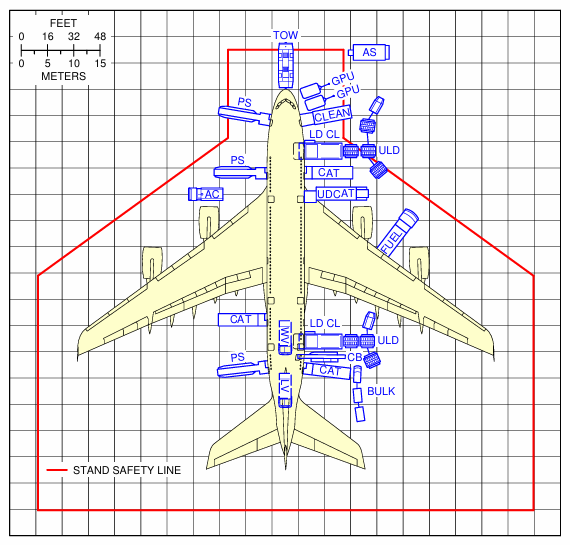
\includegraphics[width=0.8\linewidth]{Bilder/A380.png}
	\caption[Abfertigung A380]{Abfertigung eines A380 \cite{AirbusA380Characteristics}}
	\label{abfertigung}
\end{figure}

Abfertigung Frachtflugzeug?
Nach Mensen werden folgend geteilt S. 1133: